% Created by tikzDevice version 0.7.0 on 2014-10-09 04:34:25
% !TEX encoding = UTF-8 Unicode
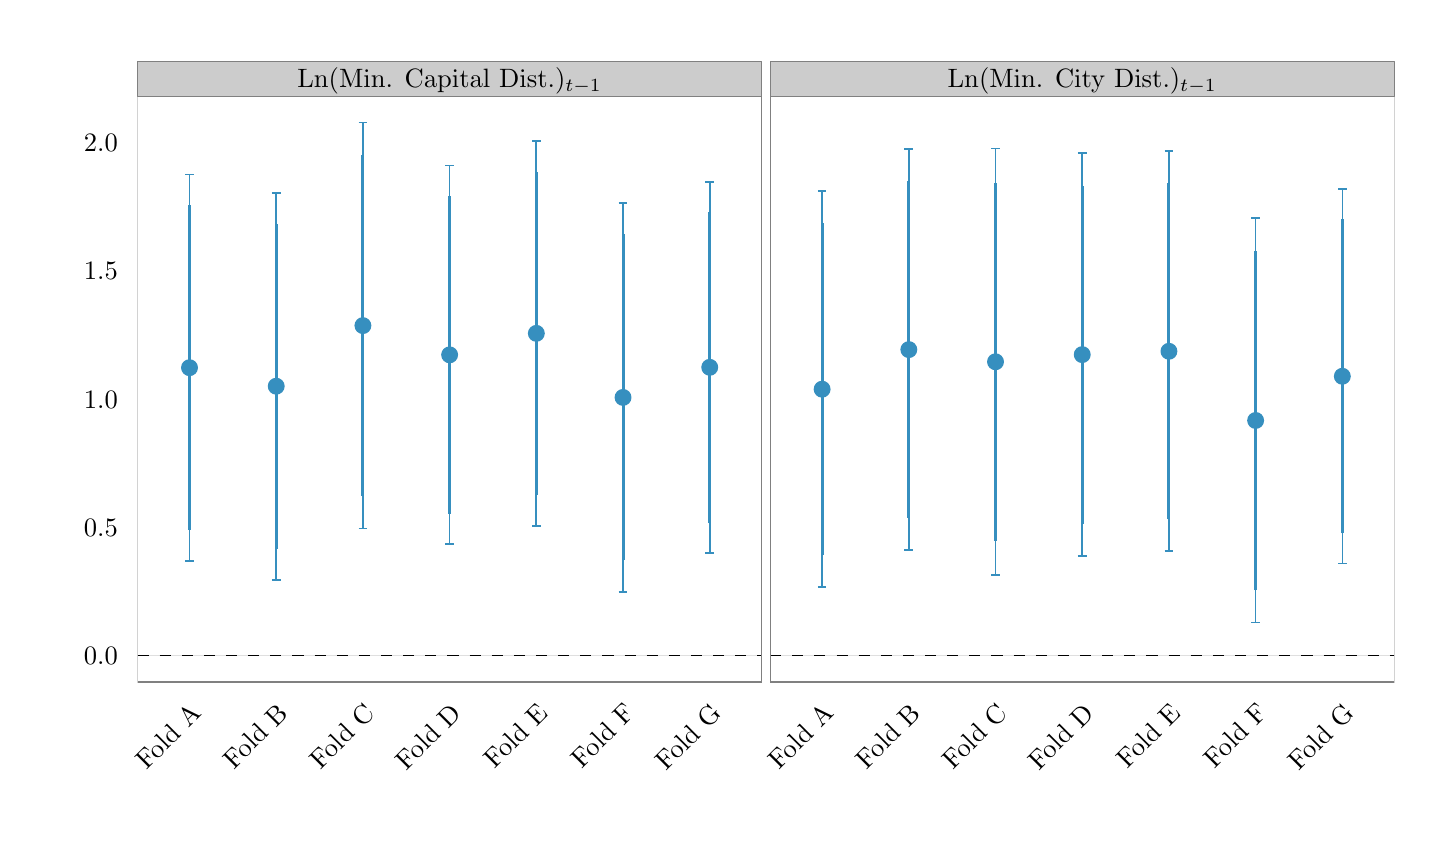
\begin{tikzpicture}[x=1pt,y=1pt]
\definecolor[named]{fillColor}{rgb}{1.00,1.00,1.00}
\path[use as bounding box,fill=fillColor,fill opacity=0.00] (0,0) rectangle (505.89,289.08);
\begin{scope}
\path[clip] (  0.00,  0.00) rectangle (505.89,289.08);
\definecolor[named]{drawColor}{rgb}{1.00,1.00,1.00}
\definecolor[named]{fillColor}{rgb}{1.00,1.00,1.00}

\path[draw=drawColor,line width= 0.6pt,line join=round,line cap=round,fill=fillColor] (  0.00,  0.00) rectangle (505.89,289.08);
\end{scope}
\begin{scope}
\path[clip] ( 39.69, 52.60) rectangle (265.26,264.40);
\definecolor[named]{fillColor}{rgb}{1.00,1.00,1.00}

\path[fill=fillColor] ( 39.69, 52.60) rectangle (265.26,264.40);
\definecolor[named]{drawColor}{rgb}{0.21,0.56,0.75}
\definecolor[named]{fillColor}{rgb}{0.21,0.56,0.75}

\path[draw=drawColor,draw opacity=0.30,line width= 0.3pt,line join=round,fill=fillColor,fill opacity=0.30] ( 58.48, 96.37) -- ( 58.48,236.07);

\path[draw=drawColor,draw opacity=0.30,line width= 0.3pt,line join=round,fill=fillColor,fill opacity=0.30] ( 89.81, 89.61) -- ( 89.81,229.43);

\path[draw=drawColor,draw opacity=0.30,line width= 0.3pt,line join=round,fill=fillColor,fill opacity=0.30] (121.14,108.07) -- (121.14,254.77);

\path[draw=drawColor,draw opacity=0.30,line width= 0.3pt,line join=round,fill=fillColor,fill opacity=0.30] (152.47,102.39) -- (152.47,239.32);

\path[draw=drawColor,draw opacity=0.30,line width= 0.3pt,line join=round,fill=fillColor,fill opacity=0.30] (183.80,109.03) -- (183.80,248.22);

\path[draw=drawColor,draw opacity=0.30,line width= 0.3pt,line join=round,fill=fillColor,fill opacity=0.30] (215.13, 85.27) -- (215.13,225.67);

\path[draw=drawColor,draw opacity=0.30,line width= 0.3pt,line join=round,fill=fillColor,fill opacity=0.30] (246.46, 99.29) -- (246.46,233.41);
\definecolor[named]{drawColor}{rgb}{0.21,0.56,0.75}
\definecolor[named]{fillColor}{rgb}{0.21,0.56,0.75}

\path[draw=drawColor,line width= 1.1pt,line join=round,fill=fillColor] ( 58.48,107.60) -- ( 58.48,224.84);

\path[draw=drawColor,line width= 1.1pt,line join=round,fill=fillColor] ( 89.81,100.85) -- ( 89.81,218.19);

\path[draw=drawColor,line width= 1.1pt,line join=round,fill=fillColor] (121.14,119.86) -- (121.14,242.98);

\path[draw=drawColor,line width= 1.1pt,line join=round,fill=fillColor] (152.47,113.40) -- (152.47,228.31);

\path[draw=drawColor,line width= 1.1pt,line join=round,fill=fillColor] (183.80,120.22) -- (183.80,237.03);

\path[draw=drawColor,line width= 1.1pt,line join=round,fill=fillColor] (215.13, 96.56) -- (215.13,214.39);

\path[draw=drawColor,line width= 1.1pt,line join=round,fill=fillColor] (246.46,110.07) -- (246.46,222.63);
\definecolor[named]{drawColor}{rgb}{0.00,0.00,0.00}
\definecolor[named]{fillColor}{rgb}{0.00,0.00,0.00}

\path[draw=drawColor,line width= 0.6pt,dash pattern=on 4pt off 4pt ,line join=round,fill=fillColor] ( 39.69, 62.23) -- (265.26, 62.23);
\definecolor[named]{drawColor}{rgb}{0.21,0.56,0.75}
\definecolor[named]{fillColor}{rgb}{0.21,0.56,0.75}

\path[draw=drawColor,line width= 0.4pt,line join=round,line cap=round,fill=fillColor] ( 58.48,166.22) circle (  2.85);

\path[draw=drawColor,line width= 0.4pt,line join=round,line cap=round,fill=fillColor] ( 89.81,159.52) circle (  2.85);

\path[draw=drawColor,line width= 0.4pt,line join=round,line cap=round,fill=fillColor] (121.14,181.42) circle (  2.85);

\path[draw=drawColor,line width= 0.4pt,line join=round,line cap=round,fill=fillColor] (152.47,170.85) circle (  2.85);

\path[draw=drawColor,line width= 0.4pt,line join=round,line cap=round,fill=fillColor] (183.80,178.62) circle (  2.85);

\path[draw=drawColor,line width= 0.4pt,line join=round,line cap=round,fill=fillColor] (215.13,155.47) circle (  2.85);

\path[draw=drawColor,line width= 0.4pt,line join=round,line cap=round,fill=fillColor] (246.46,166.35) circle (  2.85);

\path[draw=drawColor,line width= 0.6pt,line join=round] ( 56.92,236.07) --
	( 60.05,236.07);

\path[draw=drawColor,line width= 0.6pt,line join=round] ( 58.48,236.07) --
	( 58.48, 96.37);

\path[draw=drawColor,line width= 0.6pt,line join=round] ( 56.92, 96.37) --
	( 60.05, 96.37);

\path[draw=drawColor,line width= 0.6pt,line join=round] ( 88.25,229.43) --
	( 91.38,229.43);

\path[draw=drawColor,line width= 0.6pt,line join=round] ( 89.81,229.43) --
	( 89.81, 89.61);

\path[draw=drawColor,line width= 0.6pt,line join=round] ( 88.25, 89.61) --
	( 91.38, 89.61);

\path[draw=drawColor,line width= 0.6pt,line join=round] (119.58,254.77) --
	(122.71,254.77);

\path[draw=drawColor,line width= 0.6pt,line join=round] (121.14,254.77) --
	(121.14,108.07);

\path[draw=drawColor,line width= 0.6pt,line join=round] (119.58,108.07) --
	(122.71,108.07);

\path[draw=drawColor,line width= 0.6pt,line join=round] (150.91,239.32) --
	(154.04,239.32);

\path[draw=drawColor,line width= 0.6pt,line join=round] (152.47,239.32) --
	(152.47,102.39);

\path[draw=drawColor,line width= 0.6pt,line join=round] (150.91,102.39) --
	(154.04,102.39);

\path[draw=drawColor,line width= 0.6pt,line join=round] (182.24,248.22) --
	(185.37,248.22);

\path[draw=drawColor,line width= 0.6pt,line join=round] (183.80,248.22) --
	(183.80,109.03);

\path[draw=drawColor,line width= 0.6pt,line join=round] (182.24,109.03) --
	(185.37,109.03);

\path[draw=drawColor,line width= 0.6pt,line join=round] (213.57,225.67) --
	(216.70,225.67);

\path[draw=drawColor,line width= 0.6pt,line join=round] (215.13,225.67) --
	(215.13, 85.27);

\path[draw=drawColor,line width= 0.6pt,line join=round] (213.57, 85.27) --
	(216.70, 85.27);

\path[draw=drawColor,line width= 0.6pt,line join=round] (244.90,233.41) --
	(248.03,233.41);

\path[draw=drawColor,line width= 0.6pt,line join=round] (246.46,233.41) --
	(246.46, 99.29);

\path[draw=drawColor,line width= 0.6pt,line join=round] (244.90, 99.29) --
	(248.03, 99.29);
\definecolor[named]{drawColor}{rgb}{0.50,0.50,0.50}

\path[draw=drawColor,line width= 0.6pt,line join=round,line cap=round] ( 39.69, 52.60) rectangle (265.26,264.40);
\end{scope}
\begin{scope}
\path[clip] (268.27, 52.60) rectangle (493.85,264.40);
\definecolor[named]{fillColor}{rgb}{1.00,1.00,1.00}

\path[fill=fillColor] (268.27, 52.60) rectangle (493.85,264.40);
\definecolor[named]{drawColor}{rgb}{0.21,0.56,0.75}
\definecolor[named]{fillColor}{rgb}{0.21,0.56,0.75}

\path[draw=drawColor,draw opacity=0.30,line width= 0.3pt,line join=round,fill=fillColor,fill opacity=0.30] (287.07, 86.92) -- (287.07,229.97);

\path[draw=drawColor,draw opacity=0.30,line width= 0.3pt,line join=round,fill=fillColor,fill opacity=0.30] (318.40,100.36) -- (318.40,245.14);

\path[draw=drawColor,draw opacity=0.30,line width= 0.3pt,line join=round,fill=fillColor,fill opacity=0.30] (349.73, 91.30) -- (349.73,245.39);

\path[draw=drawColor,draw opacity=0.30,line width= 0.3pt,line join=round,fill=fillColor,fill opacity=0.30] (381.06, 98.14) -- (381.06,243.75);

\path[draw=drawColor,draw opacity=0.30,line width= 0.3pt,line join=round,fill=fillColor,fill opacity=0.30] (412.39, 99.88) -- (412.39,244.40);

\path[draw=drawColor,draw opacity=0.30,line width= 0.3pt,line join=round,fill=fillColor,fill opacity=0.30] (443.72, 74.08) -- (443.72,220.21);

\path[draw=drawColor,draw opacity=0.30,line width= 0.3pt,line join=round,fill=fillColor,fill opacity=0.30] (475.05, 95.45) -- (475.05,230.77);
\definecolor[named]{drawColor}{rgb}{0.21,0.56,0.75}
\definecolor[named]{fillColor}{rgb}{0.21,0.56,0.75}

\path[draw=drawColor,line width= 1.1pt,line join=round,fill=fillColor] (287.07, 98.41) -- (287.07,218.47);

\path[draw=drawColor,line width= 1.1pt,line join=round,fill=fillColor] (318.40,112.00) -- (318.40,233.50);

\path[draw=drawColor,line width= 1.1pt,line join=round,fill=fillColor] (349.73,103.69) -- (349.73,233.00);

\path[draw=drawColor,line width= 1.1pt,line join=round,fill=fillColor] (381.06,109.85) -- (381.06,232.04);

\path[draw=drawColor,line width= 1.1pt,line join=round,fill=fillColor] (412.39,111.49) -- (412.39,232.78);

\path[draw=drawColor,line width= 1.1pt,line join=round,fill=fillColor] (443.72, 85.83) -- (443.72,208.46);

\path[draw=drawColor,line width= 1.1pt,line join=round,fill=fillColor] (475.05,106.33) -- (475.05,219.89);
\definecolor[named]{drawColor}{rgb}{0.00,0.00,0.00}
\definecolor[named]{fillColor}{rgb}{0.00,0.00,0.00}

\path[draw=drawColor,line width= 0.6pt,dash pattern=on 4pt off 4pt ,line join=round,fill=fillColor] (268.27, 62.23) -- (493.85, 62.23);
\definecolor[named]{drawColor}{rgb}{0.21,0.56,0.75}
\definecolor[named]{fillColor}{rgb}{0.21,0.56,0.75}

\path[draw=drawColor,line width= 0.4pt,line join=round,line cap=round,fill=fillColor] (287.07,158.44) circle (  2.85);

\path[draw=drawColor,line width= 0.4pt,line join=round,line cap=round,fill=fillColor] (318.40,172.75) circle (  2.85);

\path[draw=drawColor,line width= 0.4pt,line join=round,line cap=round,fill=fillColor] (349.73,168.35) circle (  2.85);

\path[draw=drawColor,line width= 0.4pt,line join=round,line cap=round,fill=fillColor] (381.06,170.94) circle (  2.85);

\path[draw=drawColor,line width= 0.4pt,line join=round,line cap=round,fill=fillColor] (412.39,172.14) circle (  2.85);

\path[draw=drawColor,line width= 0.4pt,line join=round,line cap=round,fill=fillColor] (443.72,147.14) circle (  2.85);

\path[draw=drawColor,line width= 0.4pt,line join=round,line cap=round,fill=fillColor] (475.05,163.11) circle (  2.85);

\path[draw=drawColor,line width= 0.6pt,line join=round] (285.50,229.97) --
	(288.64,229.97);

\path[draw=drawColor,line width= 0.6pt,line join=round] (287.07,229.97) --
	(287.07, 86.92);

\path[draw=drawColor,line width= 0.6pt,line join=round] (285.50, 86.92) --
	(288.64, 86.92);

\path[draw=drawColor,line width= 0.6pt,line join=round] (316.83,245.14) --
	(319.97,245.14);

\path[draw=drawColor,line width= 0.6pt,line join=round] (318.40,245.14) --
	(318.40,100.36);

\path[draw=drawColor,line width= 0.6pt,line join=round] (316.83,100.36) --
	(319.97,100.36);

\path[draw=drawColor,line width= 0.6pt,line join=round] (348.16,245.39) --
	(351.30,245.39);

\path[draw=drawColor,line width= 0.6pt,line join=round] (349.73,245.39) --
	(349.73, 91.30);

\path[draw=drawColor,line width= 0.6pt,line join=round] (348.16, 91.30) --
	(351.30, 91.30);

\path[draw=drawColor,line width= 0.6pt,line join=round] (379.49,243.75) --
	(382.62,243.75);

\path[draw=drawColor,line width= 0.6pt,line join=round] (381.06,243.75) --
	(381.06, 98.14);

\path[draw=drawColor,line width= 0.6pt,line join=round] (379.49, 98.14) --
	(382.62, 98.14);

\path[draw=drawColor,line width= 0.6pt,line join=round] (410.82,244.40) --
	(413.95,244.40);

\path[draw=drawColor,line width= 0.6pt,line join=round] (412.39,244.40) --
	(412.39, 99.88);

\path[draw=drawColor,line width= 0.6pt,line join=round] (410.82, 99.88) --
	(413.95, 99.88);

\path[draw=drawColor,line width= 0.6pt,line join=round] (442.15,220.21) --
	(445.28,220.21);

\path[draw=drawColor,line width= 0.6pt,line join=round] (443.72,220.21) --
	(443.72, 74.08);

\path[draw=drawColor,line width= 0.6pt,line join=round] (442.15, 74.08) --
	(445.28, 74.08);

\path[draw=drawColor,line width= 0.6pt,line join=round] (473.48,230.77) --
	(476.61,230.77);

\path[draw=drawColor,line width= 0.6pt,line join=round] (475.05,230.77) --
	(475.05, 95.45);

\path[draw=drawColor,line width= 0.6pt,line join=round] (473.48, 95.45) --
	(476.61, 95.45);
\definecolor[named]{drawColor}{rgb}{0.50,0.50,0.50}

\path[draw=drawColor,line width= 0.6pt,line join=round,line cap=round] (268.27, 52.60) rectangle (493.85,264.40);
\end{scope}
\begin{scope}
\path[clip] (  0.00,  0.00) rectangle (505.89,289.08);
\definecolor[named]{drawColor}{rgb}{0.50,0.50,0.50}
\definecolor[named]{fillColor}{rgb}{0.80,0.80,0.80}

\path[draw=drawColor,line width= 0.2pt,line join=round,line cap=round,fill=fillColor] ( 39.69,264.40) rectangle (265.26,277.04);
\definecolor[named]{drawColor}{rgb}{0.00,0.00,0.00}

\node[text=drawColor,anchor=base,inner sep=0pt, outer sep=0pt, scale=  0.96] at (152.47,267.41) {Ln(Min. Capital Dist.)$_{t-1}$};
\end{scope}
\begin{scope}
\path[clip] (  0.00,  0.00) rectangle (505.89,289.08);
\definecolor[named]{drawColor}{rgb}{0.50,0.50,0.50}
\definecolor[named]{fillColor}{rgb}{0.80,0.80,0.80}

\path[draw=drawColor,line width= 0.2pt,line join=round,line cap=round,fill=fillColor] (268.27,264.40) rectangle (493.85,277.04);
\definecolor[named]{drawColor}{rgb}{0.00,0.00,0.00}

\node[text=drawColor,anchor=base,inner sep=0pt, outer sep=0pt, scale=  0.96] at (381.06,267.41) {Ln(Min. City Dist.)$_{t-1}$};
\end{scope}
\begin{scope}
\path[clip] (  0.00,  0.00) rectangle (505.89,289.08);
\definecolor[named]{drawColor}{rgb}{0.00,0.00,0.00}

\node[text=drawColor,anchor=base east,inner sep=0pt, outer sep=0pt, scale=  0.96] at ( 32.57, 58.92) {0.0};

\node[text=drawColor,anchor=base east,inner sep=0pt, outer sep=0pt, scale=  0.96] at ( 32.57,105.28) {0.5};

\node[text=drawColor,anchor=base east,inner sep=0pt, outer sep=0pt, scale=  0.96] at ( 32.57,151.64) {1.0};

\node[text=drawColor,anchor=base east,inner sep=0pt, outer sep=0pt, scale=  0.96] at ( 32.57,198.00) {1.5};

\node[text=drawColor,anchor=base east,inner sep=0pt, outer sep=0pt, scale=  0.96] at ( 32.57,244.36) {2.0};
\end{scope}
\begin{scope}
\path[clip] (  0.00,  0.00) rectangle (505.89,289.08);
\definecolor[named]{drawColor}{rgb}{0.00,0.00,0.00}

\node[text=drawColor,rotate= 45.00,anchor=base east,inner sep=0pt, outer sep=0pt, scale=  0.96] at ( 63.16, 40.81) {Fold A};

\node[text=drawColor,rotate= 45.00,anchor=base east,inner sep=0pt, outer sep=0pt, scale=  0.96] at ( 94.49, 40.81) {Fold B};

\node[text=drawColor,rotate= 45.00,anchor=base east,inner sep=0pt, outer sep=0pt, scale=  0.96] at (125.82, 40.81) {Fold C};

\node[text=drawColor,rotate= 45.00,anchor=base east,inner sep=0pt, outer sep=0pt, scale=  0.96] at (157.15, 40.81) {Fold D};

\node[text=drawColor,rotate= 45.00,anchor=base east,inner sep=0pt, outer sep=0pt, scale=  0.96] at (188.48, 40.81) {Fold E};

\node[text=drawColor,rotate= 45.00,anchor=base east,inner sep=0pt, outer sep=0pt, scale=  0.96] at (219.81, 40.81) {Fold F};

\node[text=drawColor,rotate= 45.00,anchor=base east,inner sep=0pt, outer sep=0pt, scale=  0.96] at (251.14, 40.81) {Fold G};
\end{scope}
\begin{scope}
\path[clip] (  0.00,  0.00) rectangle (505.89,289.08);
\definecolor[named]{drawColor}{rgb}{0.00,0.00,0.00}

\node[text=drawColor,rotate= 45.00,anchor=base east,inner sep=0pt, outer sep=0pt, scale=  0.96] at (291.74, 40.81) {Fold A};

\node[text=drawColor,rotate= 45.00,anchor=base east,inner sep=0pt, outer sep=0pt, scale=  0.96] at (323.07, 40.81) {Fold B};

\node[text=drawColor,rotate= 45.00,anchor=base east,inner sep=0pt, outer sep=0pt, scale=  0.96] at (354.40, 40.81) {Fold C};

\node[text=drawColor,rotate= 45.00,anchor=base east,inner sep=0pt, outer sep=0pt, scale=  0.96] at (385.73, 40.81) {Fold D};

\node[text=drawColor,rotate= 45.00,anchor=base east,inner sep=0pt, outer sep=0pt, scale=  0.96] at (417.06, 40.81) {Fold E};

\node[text=drawColor,rotate= 45.00,anchor=base east,inner sep=0pt, outer sep=0pt, scale=  0.96] at (448.39, 40.81) {Fold F};

\node[text=drawColor,rotate= 45.00,anchor=base east,inner sep=0pt, outer sep=0pt, scale=  0.96] at (479.72, 40.81) {Fold G};
\end{scope}
\end{tikzpicture}
